\documentclass[11pt]{article}
\usepackage[utf8]{inputenc}	% Para caracteres en español
\usepackage{amsmath,amsthm,amsfonts,amssymb,amscd}
\usepackage{multirow,booktabs}
\usepackage[table]{xcolor}
\usepackage{fullpage}
\usepackage{lastpage}
\usepackage{enumitem}
\usepackage{fancyhdr}
\usepackage{mathrsfs}
\usepackage{wrapfig}
\usepackage{setspace}
\usepackage{calc}
\usepackage{multicol}
\usepackage{cancel}
\usepackage{float}
\usepackage{physics}
\usepackage[retainorgcmds]{IEEEtrantools}
\usepackage[margin=1cm]{geometry}
\usepackage{amsmath}
\newlength{\tabcont}
\setlength{\headheight}{14pt}
\setlength{\parindent}{0.0in}
\setlength{\parskip}{0.05in}
\usepackage{empheq}
\usepackage{framed}
\usepackage[most]{tcolorbox}
\usepackage{xcolor}
\usepackage[version=3]{mhchem}
\usepackage[english]{babel}
\usepackage[utf8]{inputenc}
\usepackage{graphicx}
\usepackage[colorinlistoftodos]{todonotes}
\usepackage{mdframed}

\colorlet{shadecolor}{orange!15}
\parindent 0in
\parskip 12pt
\geometry{margin=1in, headsep=0.45in}
\theoremstyle{definition}
\newtheorem{defn}{Definition}
\newtheorem{reg}{Rule}
\newtheorem{exer}{Exercise}
\newtheorem{note}{Note}
\begin{document}
\setcounter{section}{2}
%\setcounter{subsection}{}
\title{Problem Set 8}

%==============================================================
%\thispagestyle{empty}
\pagestyle{fancy}
\fancyhf{}
\rhead{Physics 180}
\chead{Problem Set 8}
\lhead{Olyn D. Desabelle}
\rfoot{Page \thepage}

\begin{center}
{\LARGE \bf Problem Set 8}\\
%{\large Physics 180}\\
%Olyn D. Desabelle
\end{center}

\begin{figure}[H]
    \centering
    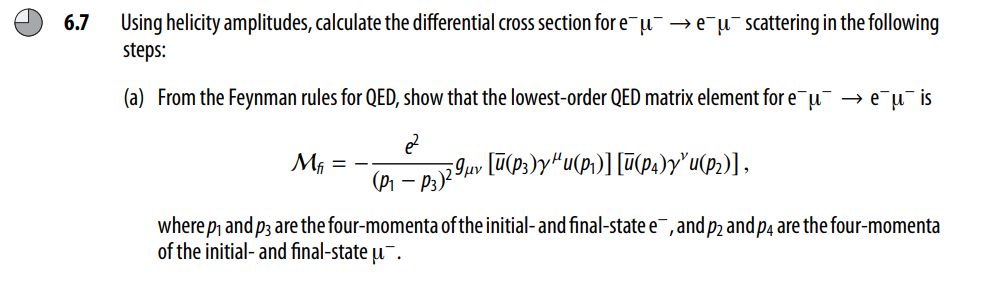
\includegraphics[scale = 0.5]{6.7a.png}
\end{figure}


For the $e^-\mu^- \to e^-\mu^-$ scattering, the Feynmann diagram will follow the $t$ configuration as such:

\begin{figure}[H]
    \centering
    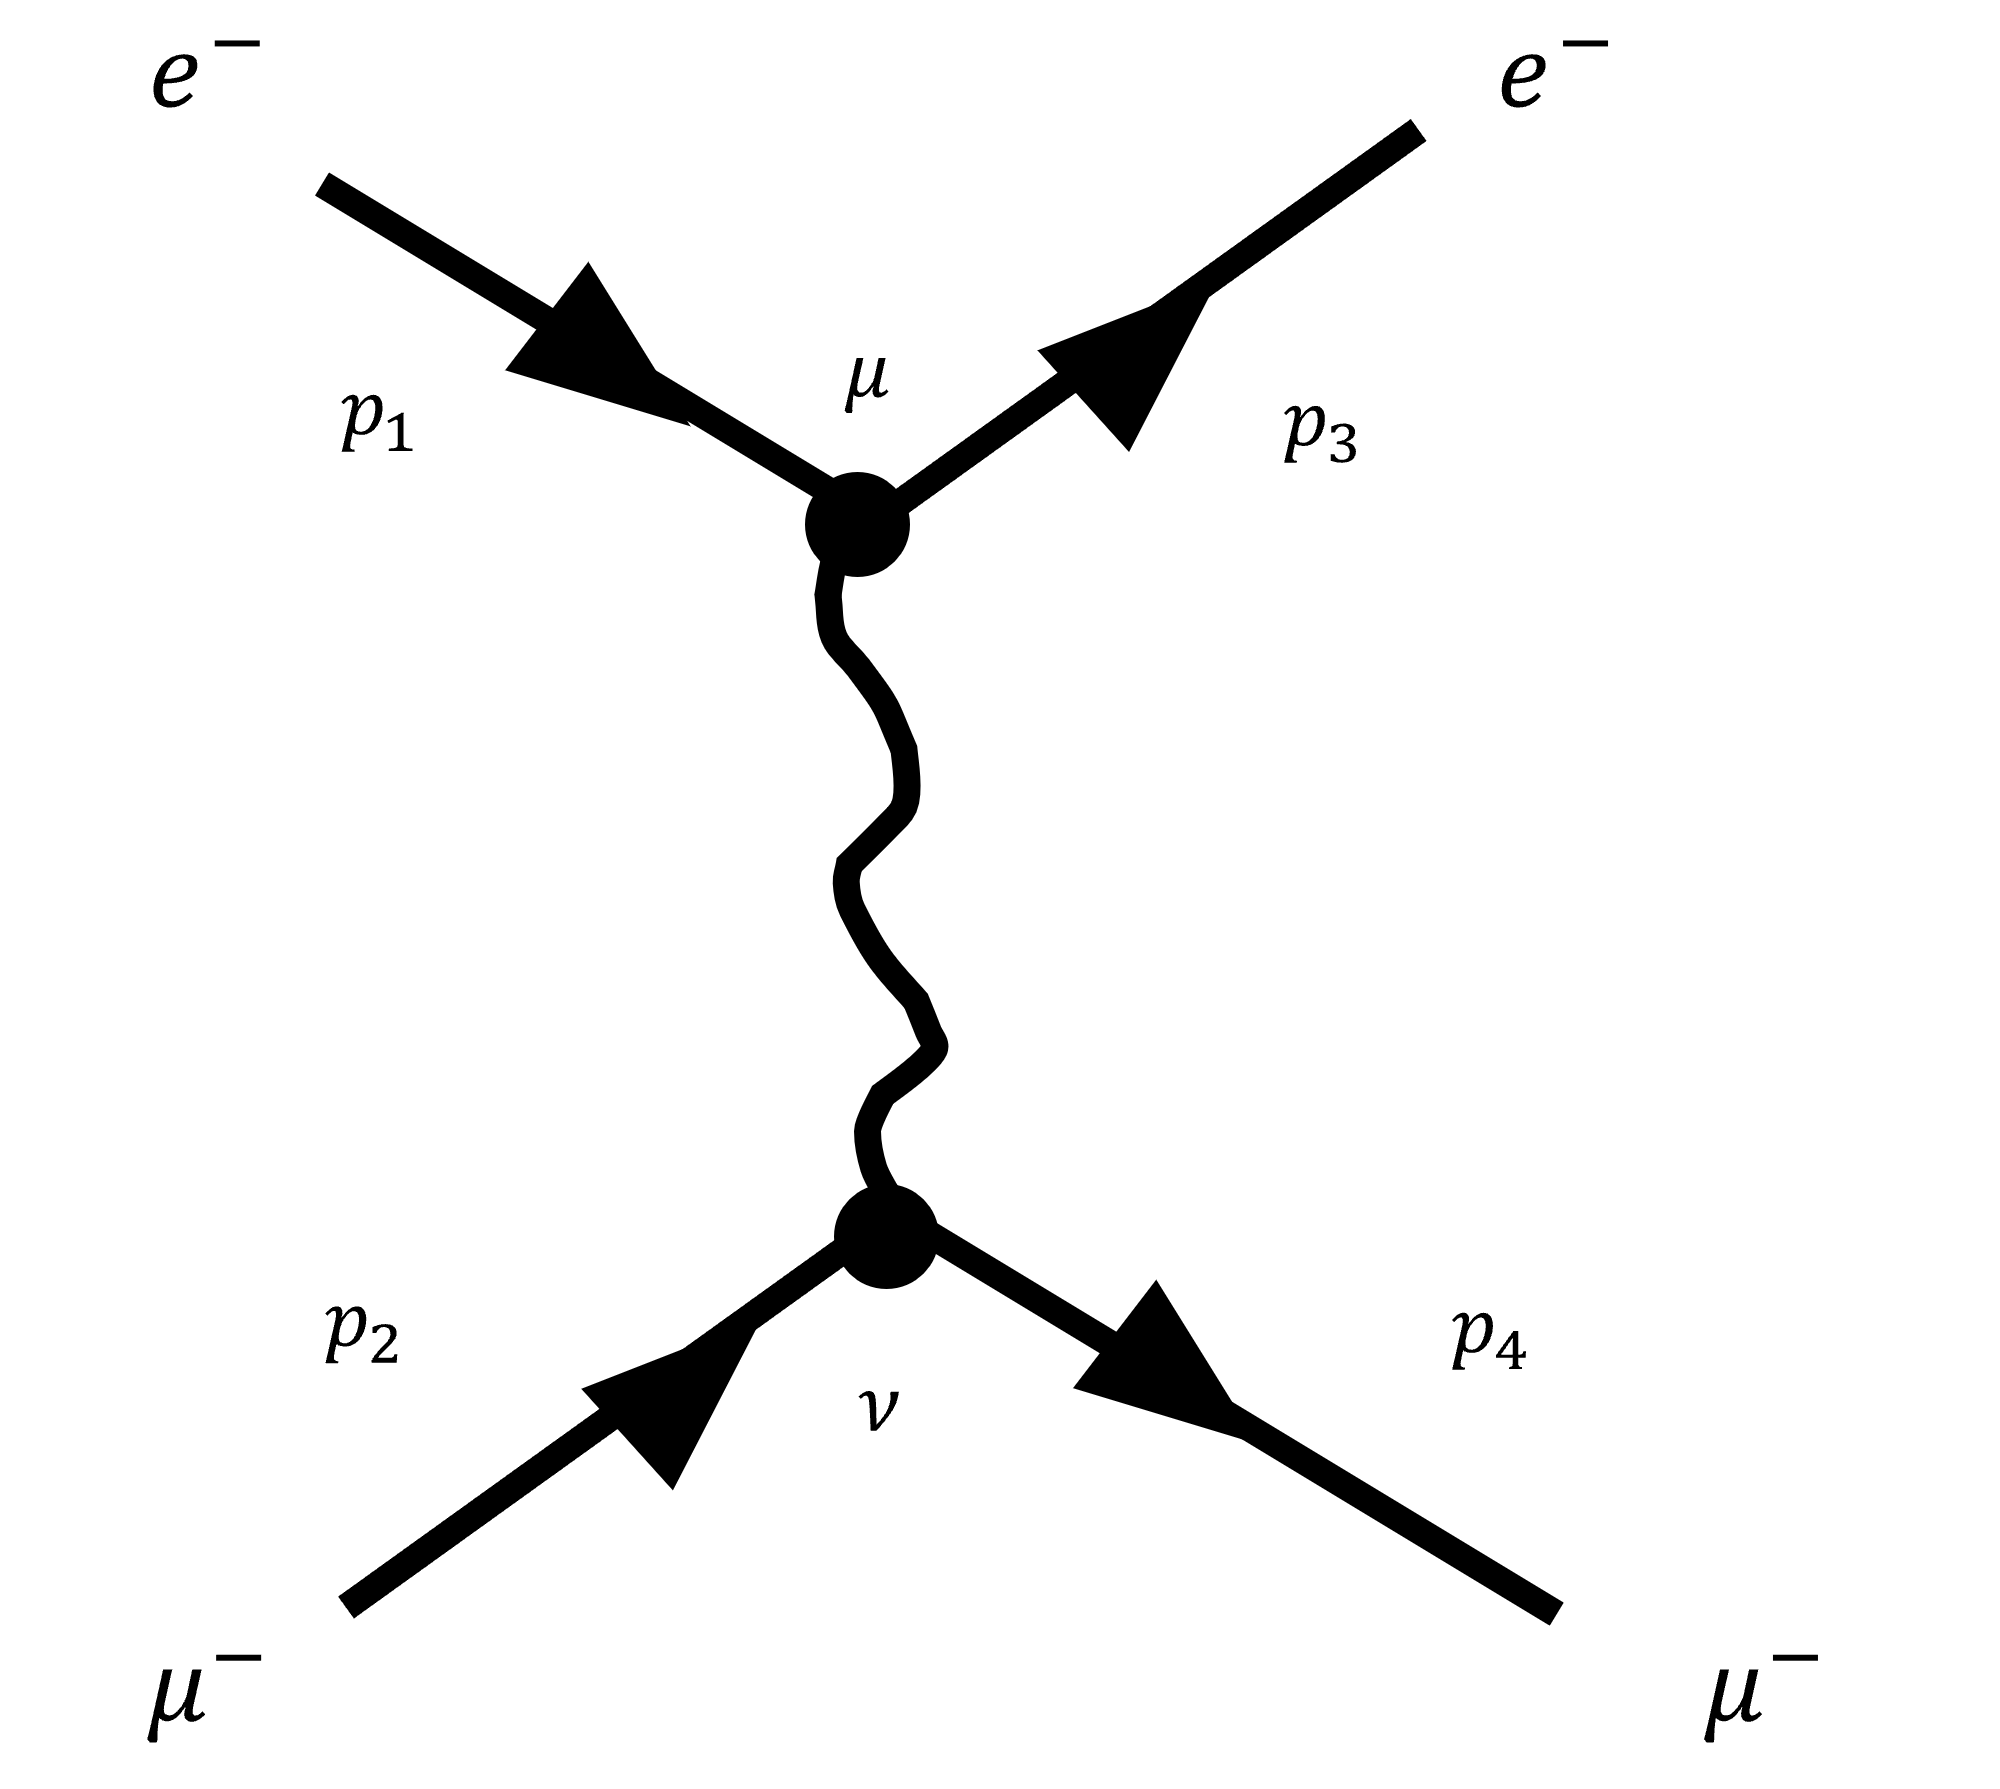
\includegraphics[scale = 0.5]{electron muon scatter.png}
\end{figure}


we recall the following from QED:

\begin{align*}
    \text{initial state particle }(e^{-}) \; &: \; u(p)\\
    \text{final state particle }(e^{-}) \; &: \; \bar{u}(p)\\
    \text{photon propagator }\; &: \; -\frac{ig_{\mu\nu}}{q^2}\\
    \text{interaction vertex factor } \; &: \; ie\gamma^{\mu}\\
\end{align*}


getting each contribution, we have the contribution from the initial state electron (particle 1) to the final state electron (particle 3):

\begin{align}
    [\bar{u}(p)]
    \left[ie\gamma^{\mu}\right]
    [u(p)]\\
    [\bar{u}(p_3)]
    \left[ie\gamma^{\mu}\right]
    [u(p_1)]\\
\end{align}

we also have sismilar contribution for the initial state muon (particle 2) and the final state muon (particle 4):


\begin{align}
    [\bar{u}(p)]
    \left[ie\gamma^{\mu}\right]
    [u(p)]\\
    [\bar{u}(p_4)]
    \left[ie\gamma^{\mu}\right]
    [u(p_2)]\\
\end{align}

combining these with the photon propagator, we then have:

\begin{align}
    -i\mathcal{M}
    &=
        [\bar{u}(p_3)]
        \left[ie\gamma^{\mu}\right]
        [u(p_1)]
    \left[
        -\frac{ig_{\mu\nu}}{q^2}
    \right]
        [\bar{u}(p_4)]
        \left[ie\gamma^{\mu}\right]
        [u(p_2)]\\
    \mathcal{M}
    &=
        -
        \frac{e^2}{q^2}
        g_{\mu\nu}
        [\bar{u}(p_3)]
        \left[\gamma^{\mu}\right]
        [u(p_1)]
        [\bar{u}(p_4)]
        \left[\gamma^{\mu}\right]
        [u(p_2)]\\
\end{align}

for the t channel configuration, $q = p_1-p_3 = p_2 - p_4$, thus we can rewrite this as:

\begin{equation}
\boxed{
    \mathcal{M}
    =
    -
        \frac{e^2}{(p_1-p_3)^2}
        g_{\mu\nu}
        [\bar{u}(p_3)
        \gamma^{\mu}
        u(p_1)]
        [\bar{u}(p_4)
        \gamma^{\mu}
        u(p_2)]
}
\end{equation}
%==============================================================
\newpage
\begin{figure}[H]
    \centering
    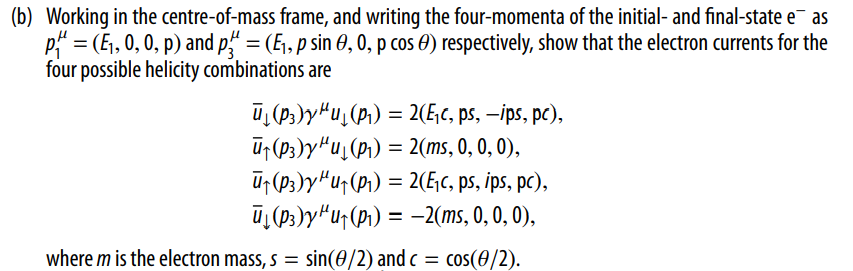
\includegraphics[scale = 0.5]{6.7b.png}
\end{figure}


The non-relativistic helicity spinors are given by Equation (4.65) of Thomson:

\begin{align}
    u_{\uparrow} =
    \sqrt{E+m}
    \begin{pmatrix}
        c\\
        se^{i\phi}\\
        \frac{p}{E+m}c\\
        \frac{p}{E+m}se^{i\phi}\\
    \end{pmatrix} \;\;\;
    u_{\downarrow} =
    \sqrt{E+m}
    \begin{pmatrix}
        -s\\
        ce^{i\phi}\\
        \frac{p}{E+m}s\\
        -\frac{p}{E+m}ce^{i\phi}\\
    \end{pmatrix}\\
\end{align}

with the given $p_1 = (E_1, 0, 0, p)$ for the incoming electron, noting that $\theta=0$ and $\phi=0$ then we have:

\begin{align}
    s = \sin(\theta/2) \to \sin(0) = 0 \;\;\;
    c = \cos(\theta/2) \to \cos(0) = 1\;\;\;
    e^{i\phi} \to e^{0} = 1
\end{align}

\begin{align}
    u_{\uparrow}(p_1) =
    \sqrt{E_1+m}
    \begin{pmatrix}
        1\\
        0\\
        \frac{p}{E_1+m}\\
        0\\
    \end{pmatrix} \;\;\;
    u_{\downarrow}(p_1) =
    \sqrt{E_1+m}
    \begin{pmatrix}
        0\\
        1\\
        0\\
        -\frac{p}{E_1+m} \\
    \end{pmatrix}\\
\end{align}


for the outgoing electron with $p_3 = (E_1, p\sin\theta, 0, p\cos\theta)$, noting that $\theta=\theta$ and $\phi=0$ we have:

\begin{align}
    s = \sin(\theta/2) \;\;\;
    c = \cos(\theta/2) \;\;\;
    e^{i\phi} \to e^{0} = 1
\end{align}

\begin{align}
    u_{\uparrow}(p_3) =
    \sqrt{E_1+m}
    \begin{pmatrix}
        c\\
        s\\
        \frac{p}{E_1+m}c\\
        \frac{p}{E_1+m}s\\
    \end{pmatrix} \;\;\;
    u_{\downarrow}(p_3) =
    \sqrt{E_1+m}
    \begin{pmatrix}
        -s\\
        c\\
        \frac{p}{E_1+m}s\\
        -\frac{p}{E_1+m}c\\
    \end{pmatrix}\\
\end{align}

we note Equations (6.12) to (6.15) of how the components of $\bar{\psi}\gamma^{\mu}\phi \equiv \psi^{\dagger}\gamma^{0}\gamma^{\mu}\phi$ may be evaluated:

\begin{align}
    \bar{\psi}\gamma^{0}\phi \equiv \psi^{\dagger}\gamma^{0}\gamma^{0}\phi &=
    \psi_1^*\phi_1 + \psi_2^*\phi_2 + \psi_3^*\phi_3 + \psi_4^*\phi_4\\
    \bar{\psi}\gamma^{1}\phi \equiv \psi^{\dagger}\gamma^{0}\gamma^{1}\phi &=
    \psi_1^*\phi_4 + \psi_2^*\phi_3 + \psi_3^*\phi_2 + \psi_4^*\phi_1\\
    \bar{\psi}\gamma^{2}\phi \equiv \psi^{\dagger}\gamma^{0}\gamma^{2}\phi &=
    -i(\psi_1^*\phi_4 - \psi_2^*\phi_3 + \psi_3^*\phi_2 - \psi_4^*\phi_1)\\
    \bar{\psi}\gamma^{3}\phi \equiv \psi^{\dagger}\gamma^{0}\gamma^{3}\phi &=
    \psi_1^*\phi_3 + \psi_2^*\phi_4 + \psi_3^*\phi_1 + \psi_4^*\phi_2\\
\end{align}

we first evaluate $\bar{u}_{\downarrow}(p_3)\gamma^{\mu}u_{\downarrow}(p_1)$ using the equations for $\bar{\psi}\gamma^{\mu}\phi \equiv \psi^{\dagger}\gamma^{0}\gamma^{\mu}\phi$:

\begin{align}
    \bar{u}_{\downarrow}(p_3)\gamma^{0}u_{\downarrow}(p_1)
    &=
    u_{\downarrow}(p_3)_1^*u_{\downarrow}(p_1)_1 + u_{\downarrow}(p_3)_2^*u_{\downarrow}(p_1)_2 + u_{\downarrow}(p_3)_3^*u_{\downarrow}(p_1)_3 + u_{\downarrow}(p_3)_4^*u_{\downarrow}(p_1)_4\\
    &= (E_1+m)\left(0 + c + \frac{cp^2}{(E_1+m)^2}\right)\\
    &\approx (2E_1-p^2)c + cp^2\\
    &= 2E_1c\\
    \bar{u}_{\downarrow}(p_3)\gamma^{1}u_{\downarrow}(p_1)
    &=
    u_{\downarrow}(p_3)_1^*u_{\downarrow}(p_1)_4 + u_{\downarrow}(p_3)_2^*u_{\downarrow}(p_1)_3 + u_{\downarrow}(p_3)_3^*u_{\downarrow}(p_1)_2 + u_{\downarrow}(p_3)_4^*u_{\downarrow}(p_1)_1\\
    &= (E_1+m) \left( \frac{sp}{E_1+m} + 0 + \frac{p}{E_1+m}s + 0 \right)\\
    &= 2ps\\
    \bar{u}_{\downarrow}(p_3)\gamma^{2}u_{\downarrow}(p_1)
    &=
    -i(u_{\downarrow}(p_3)_1^*u_{\downarrow}(p_1)_4 - u_{\downarrow}(p_3)_2^*u_{\downarrow}(p_1)_3 + u_{\downarrow}(p_3)_3^*u_{\downarrow}(p_1)_2 - u_{\downarrow}(p_3)_4^*u_{\downarrow}(p_1)_1)\\
    &= -i(E_1+m)\left( \frac{sp}{E_1+m} - 0 + \frac{p}{E_1+m}s - 0 \right)\\
    &= -2ips\\
    \bar{u}_{\downarrow}(p_3)\gamma^{3}u_{\downarrow}(p_1)
    &=
    u_{\downarrow}(p_3)_1^*u_{\downarrow}(p_1)_3 + u_{\downarrow}(p_3)_2^*u_{\downarrow}(p_1)_4 + u_{\downarrow}(p_3)_3^*u_{\downarrow}(p_1)_1 + u_{\downarrow}(p_3)_4^*u_{\downarrow}(p_1)_2\\
    &=(E_1+m) \left( 0 + \frac{-cp}{E_1+m} + 0 + \frac{-p}{E_1+m}c \right)\\
    &= 2pc
\end{align}

for the first component we used the approximation:

\begin{align}
    E^2 \approx p^2 + m \;\;\; \text{(in natural units $c=1$, and $m^2\approx m$ since $m$ is very small)}\\
\end{align}

combining all the components, we have:

\begin{equation}
\boxed{
    \bar{u}_{\downarrow}(p_3)\gamma^{\mu}u_{\downarrow}(p_1) = 
    2(E_1c, ps, -ips, pc)
}
\end{equation}

we next evaluate the components of $\bar{u}_{\uparrow}(p_3)\gamma^{\mu}u_{\downarrow}(p_1)$:

\begin{align}
    \bar{u}_{\uparrow}(p_3)\gamma^{0}u_{\downarrow}(p_1)
    &=
    u_{\uparrow}(p_3)_1^*u_{\downarrow}(p_1)_1 + u_{\uparrow}(p_3)_2^*u_{\downarrow}(p_1)_2 + u_{\uparrow}(p_3)_3^*u_{\downarrow}(p_1)_3 + u_{\uparrow}(p_3)_4^*u_{\downarrow}(p_1)_4\\
    &= (E_1+m)\left( 0 + s + 0 -\frac{p^2}{(E_1+m)^2}s\right)\\
    &\approx (2m+p^2)s - p^2s\\
    &= 2ms\\
    \bar{u}_{\uparrow}(p_3)\gamma^{1}u_{\downarrow}(p_1)
    &=
    u_{\uparrow}(p_3)_1^*u_{\downarrow}(p_1)_4 + u_{\uparrow}(p_3)_2^*u_{\downarrow}(p_1)_3 + u_{\uparrow}(p_3)_3^*u_{\downarrow}(p_1)_2 + u_{\uparrow}(p_3)_4^*u_{\downarrow}(p_1)_1\\
    &= (E_1+m) \left( -\frac{p}{E_1+m}c + 0 + \frac{p}{E_1+m}c + 0 \right)\\
    &= 0\\
    \bar{u}_{\uparrow}(p_3)\gamma^{2}u_{\downarrow}(p_1)
    &=
    -i(u_{\uparrow}(p_3)_1^*u_{\downarrow}(p_1)_4 - u_{\uparrow}(p_3)_2^*u_{\downarrow}(p_1)_3 + u_{\uparrow}(p_3)_3^*u_{\downarrow}(p_1)_2 - u_{\uparrow}(p_3)_4^*u_{\downarrow}(p_1)_1)\\
    &= -i(E_1+m)\left( -\frac{p}{E_1+m}c - 0 + \frac{p}{E_1+m}c - 0  \right)\\
    &= 0\\
    \bar{u}_{\uparrow}(p_3)\gamma^{3}u_{\downarrow}(p_1)
    &=
    u_{\uparrow}(p_3)_1^*u_{\downarrow}(p_1)_3 + u_{\uparrow}(p_3)_2^*u_{\downarrow}(p_1)_4 + u_{\uparrow}(p_3)_3^*u_{\downarrow}(p_1)_1 + u_{\uparrow}(p_3)_4^*u_{\downarrow}(p_1)_2\\
    &=(E_1+m) \left( 0 -\frac{sp}{E_1+m} + 0 + \frac{p}{E_1+m}s  \right)\\
    &= 0
\end{align}

combining all the components, we have:

\begin{equation}
\boxed{
    \bar{u}_{\uparrow}(p_3)\gamma^{\mu}u_{\downarrow}(p_1) = 
    2(ms, 0, 0, 0)
}
\end{equation}

we then evaluate the components of $\bar{u}_{\uparrow}(p_3)\gamma^{\mu}u_{\uparrow}(p_1)$:

\begin{align}
    \bar{u}_{\uparrow}(p_3)\gamma^{0}u_{\uparrow}(p_1)
    &=
    u_{\uparrow}(p_3)_1^*u_{\uparrow}(p_1)_1 + u_{\uparrow}(p_3)_2^*u_{\uparrow}(p_1)_2 + u_{\uparrow}(p_3)_3^*u_{\uparrow}(p_1)_3 + u_{\uparrow}(p_3)_4^*u_{\uparrow}(p_1)_4\\
    &= (E_1+m)\left( c + 0 + \frac{p^2}{E_1+m}c + 0 \right)\\
    &\approx (2E_1-p^2)c + p^2c\\
    &= 2E_1c\\
    \bar{u}_{\uparrow}(p_3)\gamma^{1}u_{\uparrow}(p_1)
    &=
    u_{\uparrow}(p_3)_1^*u_{\uparrow}(p_1)_4 + u_{\uparrow}(p_3)_2^*u_{\uparrow}(p_1)_3 + u_{\uparrow}(p_3)_3^*u_{\uparrow}(p_1)_2 + u_{\uparrow}(p_3)_4^*u_{\uparrow}(p_1)_1\\
    &= (E_1+m) \left( 0 + \frac{sp}{E_1+m} + 0 + \frac{p}{E_1+m}s \right)\\
    &= 2ps\\
    \bar{u}_{\uparrow}(p_3)\gamma^{2}u_{\uparrow}(p_1)
    &=
    -i(u_{\uparrow}(p_3)_1^*u_{\uparrow}(p_1)_4 - u_{\uparrow}(p_3)_2^*u_{\uparrow}(p_1)_3 + u_{\uparrow}(p_3)_3^*u_{\uparrow}(p_1)_2 - u_{\uparrow}(p_3)_4^*u_{\uparrow}(p_1)_1)\\
    &= -i(E_1+m)\left(  0 - \frac{sp}{E_1+m} + 0 - \frac{p}{E_1+m}s  \right)\\
    &= 2ips\\
    \bar{u}_{\uparrow}(p_3)\gamma^{3}u_{\uparrow}(p_1)
    &=
    u_{\uparrow}(p_3)_1^*u_{\uparrow}(p_1)_3 + u_{\uparrow}(p_3)_2^*u_{\uparrow}(p_1)_4 + u_{\uparrow}(p_3)_3^*u_{\uparrow}(p_1)_1 + u_{\uparrow}(p_3)_4^*u_{\uparrow}(p_1)_2\\
    &=(E_1+m) \left( \frac{cp}{E_1+m} + 0 + \frac{p}{E_1+m}c + 0 \right)\\
    &= 2pc
\end{align}

combining all the components, we have:

\begin{equation}
\boxed{
    \bar{u}_{\uparrow}(p_3)\gamma^{\mu}u_{\uparrow}(p_1) = 
    2(E_1c, ps, ips, pc)
}
\end{equation}

lastly evaluate the components of $\bar{u}_{\downarrow}(p_3)\gamma^{\mu}u_{\uparrow}(p_1)$:

\begin{align}
    \bar{u}_{\downarrow}(p_3)\gamma^{0}u_{\uparrow}(p_1)
    &=
    u_{\downarrow}(p_3)_1^*u_{\uparrow}(p_1)_1 + u_{\downarrow}(p_3)_2^*u_{\uparrow}(p_1)_2 + u_{\downarrow}(p_3)_3^*u_{\uparrow}(p_1)_3 + u_{\downarrow}(p_3)_4^*u_{\uparrow}(p_1)_4\\
    &= (E_1+m)\left( 0 + s + 0 - \frac{p^2}{E_1+m}s \right)\\
    &\approx (2m+p^2)s -p^2s\\
    &= -2ms\\
    \bar{u}_{\downarrow}(p_3)\gamma^{1}u_{\uparrow}(p_1)
    &=
    u_{\downarrow}(p_3)_1^*u_{\uparrow}(p_1)_4 + u_{\downarrow}(p_3)_2^*u_{\uparrow}(p_1)_3 + u_{\downarrow}(p_3)_3^*u_{\uparrow}(p_1)_2 + u_{\downarrow}(p_3)_4^*u_{\uparrow}(p_1)_1\\
    &= (E_1+m) \left( -\frac{cp}{E_1+m} + 0 + \frac{p}{E_1+m}c + 0 \right)\\
    &= 0\\
    \bar{u}_{\downarrow}(p_3)\gamma^{2}u_{\uparrow}(p_1)
    &=
    -i(u_{\downarrow}(p_3)_1^*u_{\uparrow}(p_1)_4 - u_{\downarrow}(p_3)_2^*u_{\uparrow}(p_1)_3 + u_{\downarrow}(p_3)_3^*u_{\uparrow}(p_1)_2 - u_{\downarrow}(p_3)_4^*u_{\uparrow}(p_1)_1)\\
    &= -i(E_1+m)\left(  -\frac{cp}{E_1+m} - 0 + \frac{p}{E_1+m}c - 0   \right)\\
    &= 0\\
    \bar{u}_{\downarrow}(p_3)\gamma^{3}u_{\uparrow}(p_1)
    &=
    u_{\downarrow}(p_3)_1^*u_{\uparrow}(p_1)_3 + u_{\downarrow}(p_3)_2^*u_{\uparrow}(p_1)_4 + u_{\downarrow}(p_3)_3^*u_{\uparrow}(p_1)_1 + u_{\downarrow}(p_3)_4^*u_{\uparrow}(p_1)_2\\
    &=(E_1+m) \left( 0 -\frac{sp}{E_1+m} + 0 - \frac{p}{E_1+m}s \right)\\
    &= 0
\end{align}

combining all the components, we have:

\begin{equation}
\boxed{
    \bar{u}_{\downarrow}(p_3)\gamma^{\mu}u_{\uparrow}(p_1) = 
        -2(ms, 0, 0, 0)
}
\end{equation}

thus we have the four possible helicity combinations:

\begin{equation*}
    \boxed{
    \begin{aligned}
        \bar{u}_{\downarrow}(p_3)\gamma^{\mu}u_{\downarrow}(p_1) &= 
        2(E_1c, ps, -ips, pc)\\
        \bar{u}_{\uparrow}(p_3)\gamma^{\mu}u_{\downarrow}(p_1) &= 
        2(ms, 0, 0, 0)\\
        \bar{u}_{\uparrow}(p_3)\gamma^{\mu}u_{\uparrow}(p_1) &= 
        2(E_1c, ps, ips, pc)\\
        \bar{u}_{\downarrow}(p_3)\gamma^{\mu}u_{\uparrow}(p_1) &= 
        -2(ms, 0, 0, 0)
    \end{aligned}
    }
 \end{equation*}

 %E = m+p^2
 %E = p^2 = m + p^2

%==============================================================
\newpage
\begin{figure}[H]
    \centering
    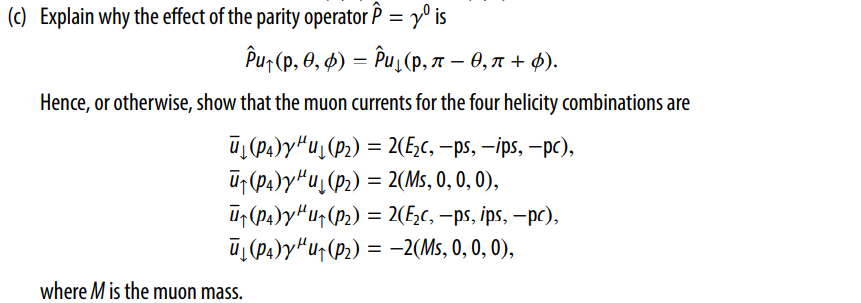
\includegraphics[scale = 0.5]{6.7c.png}
\end{figure}

We note that the parity operator $\hat{P} = \gamma^{0}$ reverses the momentum but retains spin state, such that $\hat{P}u_1(E,\mathbf{p}) = u_1(E,-\mathbf{p})$. For a given $u_{\uparrow}(p,\theta,\phi)$, having the parity operator act on it gives:

\begin{align}
    \hat{P}u_{\uparrow}(p,\theta,\phi) &= \gamma^{0}u_{\uparrow}(p,\theta,\phi)
\end{align}

we recall their Dirac-Pauli representations:

\begin{align}
    \gamma^0 =
    \begin{pmatrix}
        1 & 0 & 0 & 0\\
        0 & 1 & 0 & 0\\
        0 & 0 & -1 & 0\\
        0 & 0 & 0 & -1\\
    \end{pmatrix}
    \;\;\;\;\;
    u_{\uparrow}(p,\theta,\phi) = \sqrt{E+m}
    \begin{pmatrix}
        c\\
        se^{i\phi}\\
        \frac{p}{E+m}c\\
        \frac{p}{E+m}se^{i\phi}\\
    \end{pmatrix}
\end{align}

we then have:

\begin{align}
    \hat{P}u_{\uparrow}(p,\theta,\phi) &= 
    \begin{pmatrix}
        1 & 0 & 0 & 0\\
        0 & 1 & 0 & 0\\
        0 & 0 & -1 & 0\\
        0 & 0 & 0 & -1\\
    \end{pmatrix}
    \sqrt{E+m}
    \begin{pmatrix}
        c\\
        se^{i\phi}\\
        \frac{p}{E+m}c\\
        \frac{p}{E+m}se^{i\phi}\\
    \end{pmatrix}\\
    \hat{P}u_{\uparrow}(p,\theta,\phi) &=
    \sqrt{E+m}
    \begin{pmatrix}
        c\\
        se^{i\phi}\\
        -\frac{p}{E+m}c\\
        -\frac{p}{E+m}se^{i\phi}\\
    \end{pmatrix}\\
\end{align}

if we take a look at $u_{\downarrow}(p,\pi-\theta,\pi+\phi)$, we have:

\begin{align}
    u_{\downarrow}(p,\pi-\theta,\pi+\phi) &=
    \sqrt{E+m}
    \begin{pmatrix}
        -\sin(\frac{\pi}{2}-\frac{\theta}{2})\\
        \cos(\frac{\pi}{2}-\frac{\theta}{2})e^{i(\phi+\pi)}\\
        \frac{p}{E+m}\sin(\frac{\pi}{2}-\frac{\theta}{2})\\
        -\frac{p}{E+m}\cos(\frac{\pi}{2}-\frac{\theta}{2})e^{i(\phi+\pi)}
    \end{pmatrix}\\
    u_{\downarrow}(p,\pi-\theta,\pi+\phi) &=
    \sqrt{E+m}
    \begin{pmatrix}
        -c\\
        -se^{i\phi}\\
        \frac{p}{E+m}c\\
        \frac{p}{E+m}se^{i\phi}
    \end{pmatrix}
\end{align}

then we have the relation:

\begin{equation}
\boxed{
    \hat{P}u_{\uparrow}(p,\theta,\phi) =  u_{\downarrow}(p,\pi-\theta,\pi+\phi)
}
\end{equation}

Thus we can claim that we can get the muon currents $\bar{u}(p_4) \gamma^{\mu} u(p_2)$ from the electron currents $\bar{u}(p_3) \gamma^{\mu} u(p_1)$ such that:

\begin{align}
    \bar{u}_{\downarrow}(p_4) \gamma^{\mu} u_{\downarrow}(p_2) &= \overline{\hat{P}  u_{\uparrow}(p_3)} \gamma^{\mu} \hat{P} u_{\uparrow}(p_1)\\
    \bar{u}_{\downarrow}(p_4) \gamma^{\mu} u_{\downarrow}(p_2) &= [\hat{P}  u_{\uparrow}(p_3)]^{\dagger} \gamma^{\mu} \hat{P} u_{\uparrow}(p_1)\\
\end{align}

using the parity operator $\hat{P} = \gamma^{0}$, we have:

\begin{align}
    \bar{u}_{\downarrow}(p_4) \gamma^{\mu} u_{\downarrow}(p_2) &= [\gamma^{0} u_{\uparrow}(p_3)]^{\dagger} \gamma^{\mu} \gamma^0 u_{\uparrow}(p_1)\\
    \bar{u}_{\downarrow}(p_4) \gamma^{\mu} u_{\downarrow}(p_2) &= u_{\uparrow}^{\dagger}(p_3)\gamma^{0\dagger} \gamma^{\mu} \gamma^0 u_{\uparrow}(p_1)\\
    \bar{u}_{\downarrow}(p_4) \gamma^{\mu} u_{\downarrow}(p_2) &= \bar{u}_{\uparrow}(p_3)\gamma^{0\dagger} \gamma^{\mu} \gamma^0 u_{\uparrow}(p_1)\\
\end{align}

since we know that $\gamma^{0\dagger} = \gamma^{0}$, we then have:

\begin{align}
    \bar{u}_{\downarrow}(p_4) \gamma^{\mu} u_{\downarrow}(p_2) &= \bar{u}_{\uparrow}(p_3)\gamma^{0} \gamma^{\mu} \gamma^0 u_{\uparrow}(p_1)\\
\end{align}

in Problem Set 5, we know that:

\begin{align}
    \gamma^0\gamma^{\mu}\gamma^0  =
    \begin{cases}
        \gamma^{\mu} & \mu = 0\\
        -\gamma^{\mu} & \mu = 1,2,3
    \end{cases}
\end{align}

then we have:

\begin{align}
    \bar{u}_{\downarrow}(p_4) \gamma^{\mu} u_{\downarrow}(p_2)  =
    \begin{cases}
        \bar{u}_{\uparrow}(p_3)\gamma^{\mu} u_{\uparrow}(p_1) & \mu = 0\\
        -\bar{u}_{\uparrow}(p_3)\gamma^{\mu} u_{\uparrow}(p_1) & \mu = 1,2,3
    \end{cases}
\end{align}

meaning $\bar{u}_{\downarrow}(p_4) \gamma^{\mu} u_{\downarrow}(p_2)$ has similar 4 components with $\bar{u}_{\uparrow}(p_3)\gamma^{\mu} u_{\uparrow}(p_1)$ (the arrows reversed), but with the $\gamma^1$,$\gamma^2$, and $\gamma^3$ components multiplied by $-1$. All in all, we have:

\begin{align}
    \bar{u}_{\downarrow}(p_4) \gamma^{\mu} u_{\downarrow}(p_2) 
    &=
    \kappa(\mu)\bar{u}_{\uparrow}(p_3)\gamma^{\mu} u_{\uparrow}(p_1)\\
    \bar{u}_{\uparrow}(p_4) \gamma^{\mu} u_{\downarrow}(p_2) 
    &=
    \kappa(\mu)\bar{u}_{\downarrow}(p_3) \gamma^{\mu} u_{\uparrow}(p_1)\\
    \bar{u}_{\uparrow}(p_4) \gamma^{\mu} u_{\uparrow}(p_2)
    &=
    \kappa(\mu)\bar{u}_{\downarrow}(p_3) \gamma^{\mu} u_{\downarrow}(p_1)\\
    \bar{u}_{\downarrow}(p_4) \gamma^{\mu} u_{\uparrow}(p_2)
    &= 
    \kappa(\mu) \bar{u}_{\uparrow}(p_3) \gamma^{\mu} u_{\downarrow}(p_1)\\
\end{align}

where: %$\kappa(\mu=0) = 1$ and $\kappa(\mu=1) = \kappa(\mu=2) = \kappa(\mu=3) = -1$.

\begin{align}
    \kappa(\mu)  =
    \begin{cases}
        1 & \mu = 0\\
        -1 & \mu = 1,2,3
    \end{cases}
\end{align}

applying this to what we obtained earlier, then we get the expected helicity combinations (replacing $m$ with $M$ and $E_1$ with $E_2$) :

\begin{equation*}
\boxed{
    \begin{aligned}
    \bar{u}_{\downarrow}(p_4) \gamma^{\mu} u_{\downarrow}(p_2) 
    &=
    2(E_2c, -ps -ips, -pc)\\
    \bar{u}_{\uparrow}(p_4) \gamma^{\mu} u_{\downarrow}(p_2) 
    &=
    2(Ms, 0, 0, 0)\\
    \bar{u}_{\uparrow}(p_4) \gamma^{\mu} u_{\uparrow}(p_2)
    &=
    2(E_2c, -ps, ips, -pc)\\
    \bar{u}_{\downarrow}(p_4) \gamma^{\mu} u_{\uparrow}(p_2)
    &= 
    -2(Ms,0,0,0)\\
    \end{aligned}
}
\end{equation*}

%Recalling the non-relativistic helicity spinors given by Equation (4.65) of Thomson, we have:

%\begin{align}
%    u_{\uparrow} (p, \theta,\phi) =
%    \sqrt{E+m}
%    \begin{pmatrix}
%        c\\
%        se^{i\phi}\\
%        \frac{p}{E+m}c\\
%        \frac{p}{E+m}se^{i\phi}\\
%    \end{pmatrix} \;\;\;
%    u_{\downarrow} (p, \theta,\phi) =
%    \sqrt{E+m}
%    \begin{pmatrix}
%       -s\\
%        ce^{i\phi}\\
%        \frac{p}{E+m}s\\
%        -\frac{p}{E+m}ce^{i\phi}\\
%    \end{pmatrix}\\
%\end{align}

%we recall that:

%\begin{align}
    %\sin\left(\frac{\pi-\theta}{2}\right) = \cos\left(\frac{\theta}{2}\right), \;\;\;\;\;
    %\cos\left(\frac{\pi-\theta}{2}\right) = \sin\left(\frac{\theta}{2}\right)
%\end{align}

%thus we have:

% s = \sin(\theta/2), c= \cos(\theta/2)

%\begin{align}
  %  u_{\downarrow} (p, \pi-\theta,\pi+\phi) =
  %  \sqrt{E+m}
  %  \begin{pmatrix}
  %      -c\\
  %      se^{i(\pi+\phi)}\\
  %      \frac{p}{E+m}c\\
 %       -\frac{p}{E+m}se^{i(\pi+\phi)}\\
%    \end{pmatrix}\\
%\end{align}



%==============================================================
\newpage
\begin{figure}[H]
    \centering
    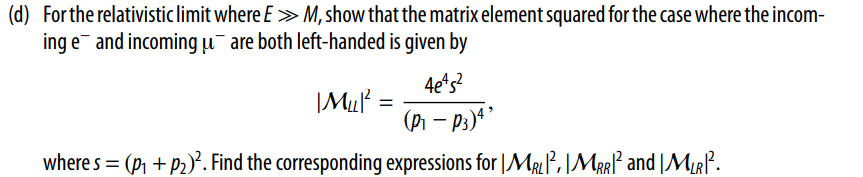
\includegraphics[scale = 0.5]{6.7d.png}
\end{figure}

Ifn the relativistic limit ($M$ and $m$ are negligible, $p = E$), then from what we have obtained, with $E_1=E_2=E$, we have for the electron current $j_e$:

\begin{align}
    j_{e,LL} &=
        \bar{u}_{\downarrow}(p_3)\gamma^{\mu}u_{\downarrow}(p_1) = 
        2E(c, s, -is, c)\\
    j_{e,RR} &=
        \bar{u}_{\uparrow}(p_3)\gamma^{\mu}u_{\uparrow}(p_1) = 
        2E(c, s, is, c)
\end{align}

for the muon current $j_{\mu}$ we have:

\begin{align}
    j_{\mu,LL} &=
    \bar{u}_{\downarrow}(p_4) \gamma^{\mu} u_{\downarrow}(p_2) 
            =
            2E(c, -s, -is, -c)\\
    j_{\mu,RR} &=
    \bar{u}_{\uparrow}(p_4) \gamma^{\mu} u_{\uparrow}(p_2)
            =
            2E(c, -s, is, -c)\\    
\end{align}

using these currents we may obtain the matrix element squared. We may first get $|\mathcal{M}_{LL}|^2$:

\begin{align}
    |\mathcal{M}_{LL}|^2 &= \left[-\frac{e^2}{t^2}j_{e,LL} \cdot j_{\mu,LL}\right]^2\\
    &= \frac{e^4}{(p_1-p_3)^4}\left[2E(c, s, -is, c) \cdot 2E(c, -s, -is, -c)\right]^2\\
    &= \frac{e^4}{(p_1-p_3)^4}\left[4E^2(c^2 + s^2 + s^2 + c^2)\right]^2
\end{align}

with $s=4E^2$ (taken from Chapter 6.2.4), this becomes:

\begin{align}
    |\mathcal{M}_{LL}|^2 &=
    \frac{e^4}{(p_1-p_3)^4}
    \left[s(2)\right]^2
\end{align}

\begin{equation}
\boxed{
    |\mathcal{M}_{LL}|^2
    =
    \frac{4e^4s^2}{(p_1-p_3)^4}
}
\end{equation}

next we try for $|\mathcal{M}_{RR}|^2$

\begin{align}
    |\mathcal{M}_{RR}|^2
    &= 
    \left[-\frac{e^2}{t^2}j_{e,RR} \cdot j_{\mu,RR}\right]^2\\
    &= \frac{e^4}{(p_1-p_3)^4}\left[2E(c, s, is, c) \cdot 2E(c, -s, is, -c)\right]^2\\
    &= \frac{e^4}{(p_1-p_3)^4}\left[4E^2(c^2 + s^2 + s^2 + c^2)\right]^2\\
    &= \frac{e^4}{(p_1-p_3)^4}
    \left[s(2)\right]^2
\end{align}

\begin{equation}
    \boxed{
        |\mathcal{M}_{RR}|^2
        =
        \frac{4e^4s^2}{(p_1-p_3)^4}
    }
\end{equation}


we proceed to the other matrix element squared, with $|\mathcal{M}_{LR}|^2$ and $|\mathcal{M}_{RL}|^2$:

\begin{align}
    |\mathcal{M}_{LR}|^2 &= \left[-\frac{e^2}{t^2}j_{e,LL} \cdot j_{\mu,RR}\right]^2\\
    &= \frac{e^4}{(p_1-p_3)^4} \left[ 2E(c, s, -is, c) \cdot 2E(c, -s, is, -c) \right]^2\\
    &= \frac{e^4}{(p_1-p_3)^4} \left[ 4E^2 (c^2 + s^2 - s^2 +c^2) \right]^2\\
    &= \frac{e^4}{(p_1-p_3)^4} \left[ s (2c^2) \right]^2 \\
\end{align}


\begin{equation}
\boxed{
    |\mathcal{M}_{LR}|^2
    =
    \frac{e^4s^2}{(p_1-p_3)^4}
    (1+\cos\theta)
}
\end{equation}

\begin{align}
    |\mathcal{M}_{RL}|^2 &= \left[-\frac{e^2}{t^2}j_{e,RR} \cdot j_{\mu,LL}\right]^2\\
    &= \frac{e^4}{(p_1-p_3)^4} \left[ 2E(c, s, is, c) \cdot 2E(c, -s, -is, -c) \right]^2\\
    &= \frac{e^4}{(p_1-p_3)^4} \left[ 4E^2 (c^2 + s^2 - s^2 +c^2) \right]^2\\
    &= \frac{e^4}{(p_1-p_3)^4} \left[ s (2c^2) \right]^2 \\
\end{align}

\begin{equation}
\boxed{
    |\mathcal{M}_{RL}|^2
    =
    \frac{e^4s^2}{(p_1-p_3)^4}
    (1+\cos\theta)
}
\end{equation}

%==============================================================
%\newpage
%\begin{figure}[H]
%    \centering
%    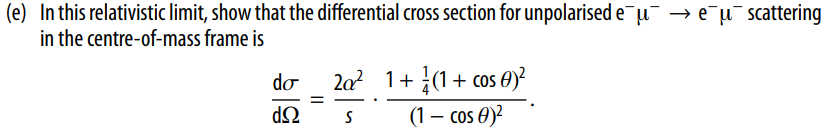
\includegraphics[scale = 0.5]{6.7e.png}
%\end{figure}

%for the cross section, we have the general formula of:

%\begin{align}
    %\frac{d\sigma}{d\Omega} = \frac{1}{64\pi^2s}\expval{|\mathcal{M}|^2}
%\end{align}

%taking the spin-averaged matrix element squared, we have:

%\begin{align}
    %\expval{|\mathcal{M}|^2} &=
    %\frac{1}{4} (|\mathcal{M}_{RR}|^2 + |\mathcal{M}_{LL}|^2 + |\mathcal{M}_{RL}|^2 + |\mathcal{M}_{LR}|^2)\\
    %&= \frac{1}{4} \left( \frac{8e^4s^2}{(p_1-p_3)^4} + 2\frac{e^4s^2}{(p_1-p_3)^4}
    %(1+\cos\theta)
    %\right)\\
    %&= \frac{2e^2s^2}{(p_1-p_3)^4}
    %\left[ 1+\frac{1}{4}(1+\cos\theta) \right]
%\end{align}

%thus our cross section becomes:

%\begin{align}
    %\frac{d\sigma}{d\Omega} = \frac{1}{64\pi^2s}
    %\frac{2e^2s^2}{(p_1-p_3)^4}
    %\left[ 1+\frac{1}{4}(1+\cos\theta) \right]
%\end{align}

%in the relativistic limit, we the electron mass is negligible and we may approximate $(p_1-p_3)^2$ as:

%\begin{align}
%    (p_1-p_3)^2
%    \approx
%    -2E^2(1-\cos\theta)  
%\end{align}
%==============================================================
\end{document}